%%%%%%%%%%%%%%%%%%%%%%%%%%%%%%%%%%%%%%%%%%%%%%%%%%%%%%%%%%%%%%%%%%
%%%%%%%% ICML 2014 EXAMPLE LATEX SUBMISSION FILE %%%%%%%%%%%%%%%%%
%%%%%%%%%%%%%%%%%%%%%%%%%%%%%%%%%%%%%%%%%%%%%%%%%%%%%%%%%%%%%%%%%%

% Use the following line _only_ if you're still using LaTeX 2.09.
%\documentstyle[icml2014,epsf,natbib]{article}
% If you rely on Latex2e packages, like most moden people use this:
\documentclass{article}


% use Times
\usepackage{times}
\usepackage{geometry,amsmath}

% For figures
\usepackage{graphicx} % more modern
%\usepackage{epsfig} % less modern
\usepackage{subfigure} 


% For citations
\usepackage{natbib}

% For algorithms
\usepackage{algorithm}
\usepackage{algorithmic}

% As of 2011, we use the hyperref package to produce hyperlinks in the
% resulting PDF.  If this breaks your system, please commend out the
% following usepackage line and replace \usepackage{icml2014} with
% \usepackage[nohyperref]{icml2014} above.
\usepackage{hyperref}

% Packages hyperref and algorithmic misbehave sometimes.  We can fix
% this with the following command.
\newcommand{\theHalgorithm}{\arabic{algorithm}}

% Employ the following version of the ``usepackage'' statement for
% submitting the draft version of the paper for review.  This will set
% the note in the first column to ``Under review.  Do not distribute.''
\usepackage{icml2014}


% The \icmltitle you define below is probably too long as a header.
% Therefore, a short form for the running title is supplied here:
\icmltitlerunning{de Villalobos, Lautman, Yim}

%%%%%%%%%% Start TeXmacs macros
\newcommand{\nosymbol}{}
\newcommand{\tmop}[1]{\ensuremath{\operatorname{#1}}}
%%%%%%%%%% End TeXmacs macros

\begin{document} 

\twocolumn[
\icmltitle{Penn Project Report\\Machine Learning in Real Time Character Recognition}

% It is OKAY to include author information, even for blind
% submissions: the style file will automatically remove it for you
% unless you've provided the [accepted] option to the icml2014
% package.
\icmlauthor{Francisco de Villalobos}{frade@seas.upenn.edu}
\icmlauthor{Michael Lautman}{mlautman@seas.upenn.edu}
\icmlauthor{Justin Yim}{yimj@seas.upenn.edu}

% You may provide any keywords that you 
% find helpful for describing your paper; these are used to populate 
% the "keywords" metadata in the PDF but will not be shown in the document
\icmlkeywords{machine learning, character recognition, kaman filter}


\vskip 0.3in
]

\begin{abstract} 
This paper presents a MEMS based digital pen for handwriting recognition. While there are several devices which are capable of digitizing handwritten notes, all commercially available devices require secondary hardware to function. We propose a single device solution for digitizing text as it is written on a page. Our device tracks position and angle and uses machine learning methods to identify written characters in real time. By solving for the dynamics of the system, and using them in our Kalman Filter, we are able to estimate the pen tip position as a function of time that will be used as inputs to a classification algorithm.
%Implementation and design of machine learning algorithms to learn characters in real time through IMU and gyro acquisitions on a regular pen.
\end{abstract} 



\section{Prototype}
In this section we give a brief summary of the hardware incorporated into the proposed device. We first describe the mechanical device before then discussing the electronics. 

\subsection{Hardware}
The pen layout and body was designed in CAD (pictured below) to ensure appropriate packing of components. The clear body was 3D printed in ABS in the University's prototyping labs. The ink for the pen rests on a small limit switch which is engaged when the user makes contact with the page. 

\begin{figure}[H]
	\centering
	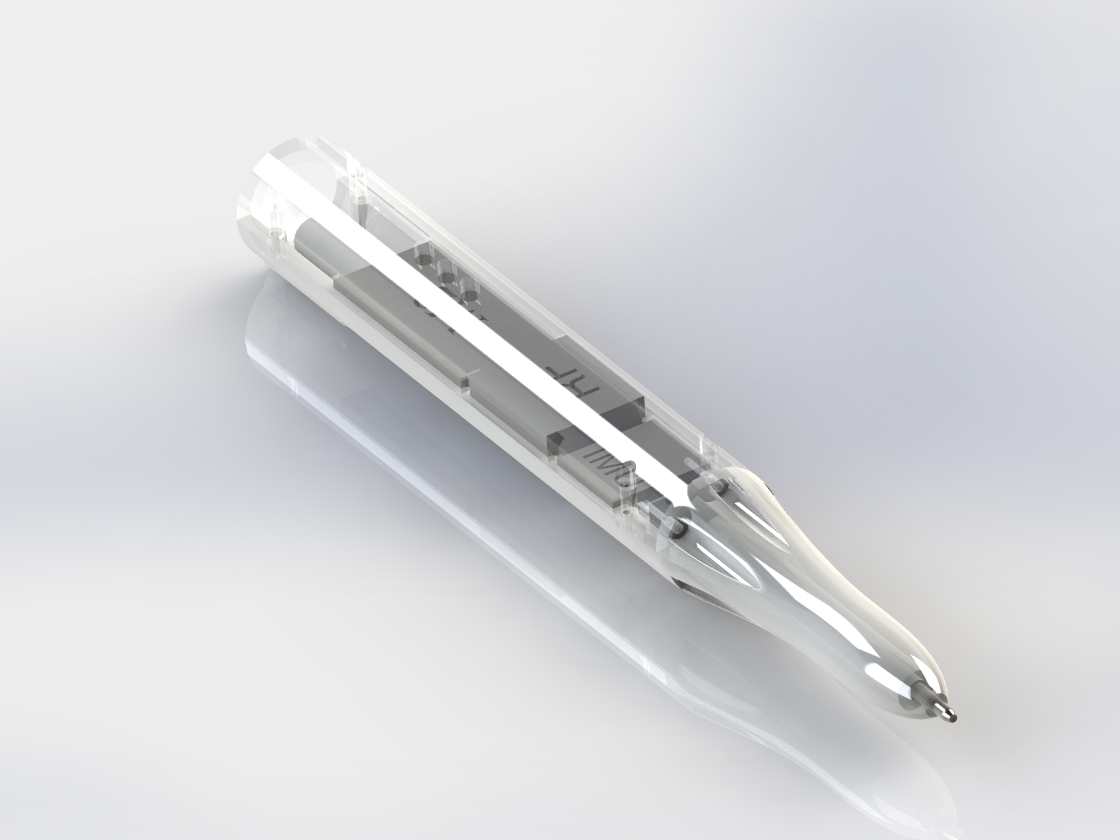
\includegraphics[width=0.5\textwidth, height= 5cm]{pen_render.png}
	\caption{Rendering of the 3D printed model of the penn}
\end{figure}

\subsection{Electronics}
An ATMega32u4 microcontroller provides on-board processing and interfaces to the wireless module, IMU, switch, and indicator LEDs. Two Nordic nRF24LE1 transceivers handle wireless communication between the pen and base station computer. Inertial measurements are provided by an MPU6050 digital IMU with configurable gain triaxial accelerometers and gyroscopes. A Honeywell HMC5883L triaxial magnetometer provides a reference to earth's magnetic field for orientation. A switch behind the pen tip detects contact with the page for character segmentation. Three LEDs on the case display pen state. The pen also includes on-board batteries, power management, and an on-off switch.
%We designed and built a custom electronic pen to gather data for character identification. Three dimensional acceleration and angular velocity measurements from the pen are streamed to a computer for processing.  Our design of the pen hardware focused on fitting inertial measurement, processing, communication, and power management into a streamlined and easy to use form.
%This stage consisted mainly of the design of a working prototype to start the data gathering process. The challenge consisted in having a non bulky pen that could stream gyro and IMU data through WiFi to the computer so that the data could then be processed by a more powerful computer.


%We first took all the ideas and components we needed to make this project work, and carried them on to sketches. Once we were pretty sure of the feasibility of the design and that it could contain everything we needed, we stepped into 3D designing a pen that could be easily 3D printed and could be manufactured rather quickly we the resources we have in AddLab. The result of the first version of the pen looks like this:


%As you can see, we have an on-board microprocessor, 3 axis accelerometer, 3 axis gyroscope, magnetometer, and WiFi module. It also has a very sensitive switch that can tel us when the pen is actually writing. On top of that, the pen has 3 LED lights to make a visual recognition of the states the pen was at. We also included in the real version, a switch to turn it on and off, and batteries.


\subsection{Filtering the data}

The raw data from the IMU pose issues for learning algorithms. Sources of variance can include posture, handed-ness, roll angle of the pen, and sensor drift. To minimize sources of error, we compute the trajectory of the pen tip on the page. Using various filtering and sensor fusion techniques we are able to compensate for gravity and perform attitude and position estimation. We use a Kalman Filter to estimate the orientation of the pen relative to gravity so that we can subtract the gravity components from the acceleration measurements. 


\subsection{Implicated Dynamics}
\textbf{P}: location of the IMU \\
\textbf{O}: origin of frame G on the page \\
\textbf{frame G}: SRT fixed to the page with origin O (ground frame) \\
\textbf{frame M}: SRT fixed to the pen at the IMU with origin at point P (pen frame) \\
\textbf{Q}: location of the pen tip \\
$\underset{\mbox{\textasciitilde}}{\tmop{\textbf{PQ}}}$: vector from the IMU origin to
the pen tip

The acceleration of the pen tip in the ground frame is given by:
\begin{align*}
  ^G \underset{\mbox{\textasciitilde}}{a}^Q =^G
  \underset{\mbox{\textasciitilde}}{a}^P +^M
  \underset{\mbox{\textasciitilde}}{a}^Q &+^G
  \underset{\mbox{\textasciitilde}}{\alpha}^P \times
  \underset{\mbox{\textasciitilde}}{\tmop{PQ}} + 2^G
  \underset{\mbox{\textasciitilde}}{w}^M \times^M
  \underset{\mbox{\textasciitilde}}{v}^Q + ... \\ &+ ^G 
  \underset{\mbox{\textasciitilde}}{w}^M \times \left(^G
  \underset{\mbox{\textasciitilde}}{w}^M \times
  \underset{\mbox{\textasciitilde}}{\tmop{PQ}} \right)
\end{align*}
Since point Q (the pen tip) is fixed in frame M (the pen frame), $^M
\underset{\mbox{\textasciitilde}}{a}^Q$ and $^M
\underset{\mbox{\textasciitilde}}{v}^Q$ are both 0. The above equation
simplifies to:
\begin{eqnarray*}
  & ^G \underset{\mbox{\textasciitilde}}{a}^Q =^G
  \underset{\mbox{\textasciitilde}}{a}^P +^G
  \underset{\mbox{\textasciitilde}}{\alpha}^P \times
  \underset{\mbox{\textasciitilde}}{\tmop{PQ}} +^G
  \underset{\mbox{\textasciitilde}}{w}^M \times \left(^G
  \underset{\mbox{\textasciitilde}}{w}^M \times
  \underset{\mbox{\textasciitilde}}{\tmop{PQ}} \right) & 
\end{eqnarray*}
The IMU measures accelerations and angular velocities of frame M relative to
frame G expressed in frame M. \ Using the attitude estimate, these
measurements can be rotated into frame G to produce $^G
\underset{\mbox{\textasciitilde}}{a}^P$ and $^G
\underset{\mbox{\textasciitilde}}{w}^M \nosymbol$. \ The angular acceleration
$^G \underset{\mbox{\textasciitilde}}{\alpha}^P$ is obtained by numerically
differentiating $^G \underset{\mbox{\textasciitilde}}{w}^M$.

The trajectory of the pen tip in the page frame is obtained by
twice-integrating $^G \underset{\mbox{\textasciitilde}}{a}^Q$.

Differentiation of $^G \underset{\mbox{\textasciitilde}}{w}^M$ greatly increases
high-frequency noise in the acceleration which is smoothed out using a low-pass
filter. Double-integration of the acceleration estimate results in drift error as small errors sum to large velocity and position errors. We use high-pass filters to remove some of the drift but there are still significant distortions apparent in the recovered trajectories. 

\subsection{Preliminary Results}
We are currently able to produce relatively accurate trajectory estimates. Figure 2 shows a trajectory recovered 'g' that we were able to produce using our methodology.

\begin{figure}[H]
\centering
    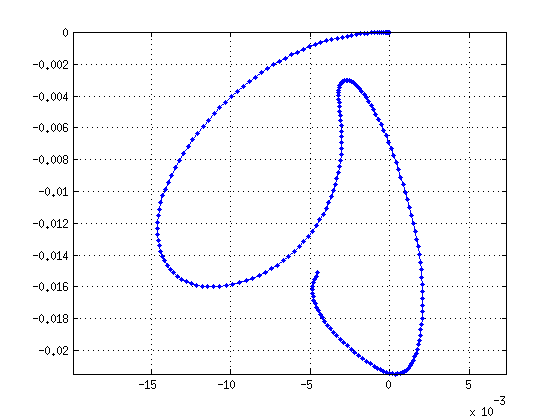
\includegraphics[width=0.5\textwidth, height= 5cm]{g.png}
    \caption{Representation results of the letter "g"}
\end{figure}


\subsection{Next Steps}
The next step in the project is to create a labeled test set. With a training set in hand, we will begin testing different learning algorithms so that we can find the most successful model. To this end, we will approach the learning component of this project in two ways. One method involves projecting the trajectory into an image and using learning algorithms such as neural networks. The other method involves using feature selection methods on the filtered signals before integration and differentiation. This method will require that we transform the time series data into a constant width feature vector. By interpolating, we are able to produce this result. Reducing dimensionality might prove to be an important step if we experience performance issues. In that case we intend to use either PCA or LDA to generate features. We intend to test the performance of various learning algorithms including Hidden Markov Models, Neural Networks, and Naive Bayes.
 
\section*{Acknowledgments} 
 
Attitude estimation Kalman Filter and initial approximation provided by \textbf{open-source} code from Sebastian Madgwick (July 2012), based on his paper \textbf{Estimation of IMU and MARG orientation using a gradient descent algorithm}.\\\\
For trajectory reconstruction, consulted Jeen-Shing Wang, Yu-Liang Hsu, and Jiun-Nan Liu's paper entitled \textbf{An Inertial-Measurement-Unit-Based Pen With a Trajectory Reconstruction Algorithm and Its Applications}.
\bibliography{example_paper}
\bibliographystyle{icml2014}

\end{document} 


% This document was modified from the file originally made available by
% Pat Langley and Andrea Danyluk for ICML-2K. This version was
% created by Lise Getoor and Tobias Scheffer, it was slightly modified  
% from the 2010 version by Thorsten Joachims & Johannes Fuernkranz, 
% slightly modified from the 2009 version by Kiri Wagstaff and 
% Sam Roweis's 2008 version, which is slightly modified from 
% Prasad Tadepalli's 2007 version which is a lightly 
% changed version of the previous year's version by Andrew Moore, 
% which was in turn edited from those of Kristian Kersting and 
% Codrina Lauth. Alex Smola contributed to the algorithmic style files.  
